%!TEX root=../../main.tex

\subsubsection{Breadth-first search}
As with our results for SSSP, for BFS we will begin with our single-node results before looking at the distributed scenario. 

\paragraph{Single-Node}
\begin{figure*}
	\begin{subfigure}{0.32\textwidth}
		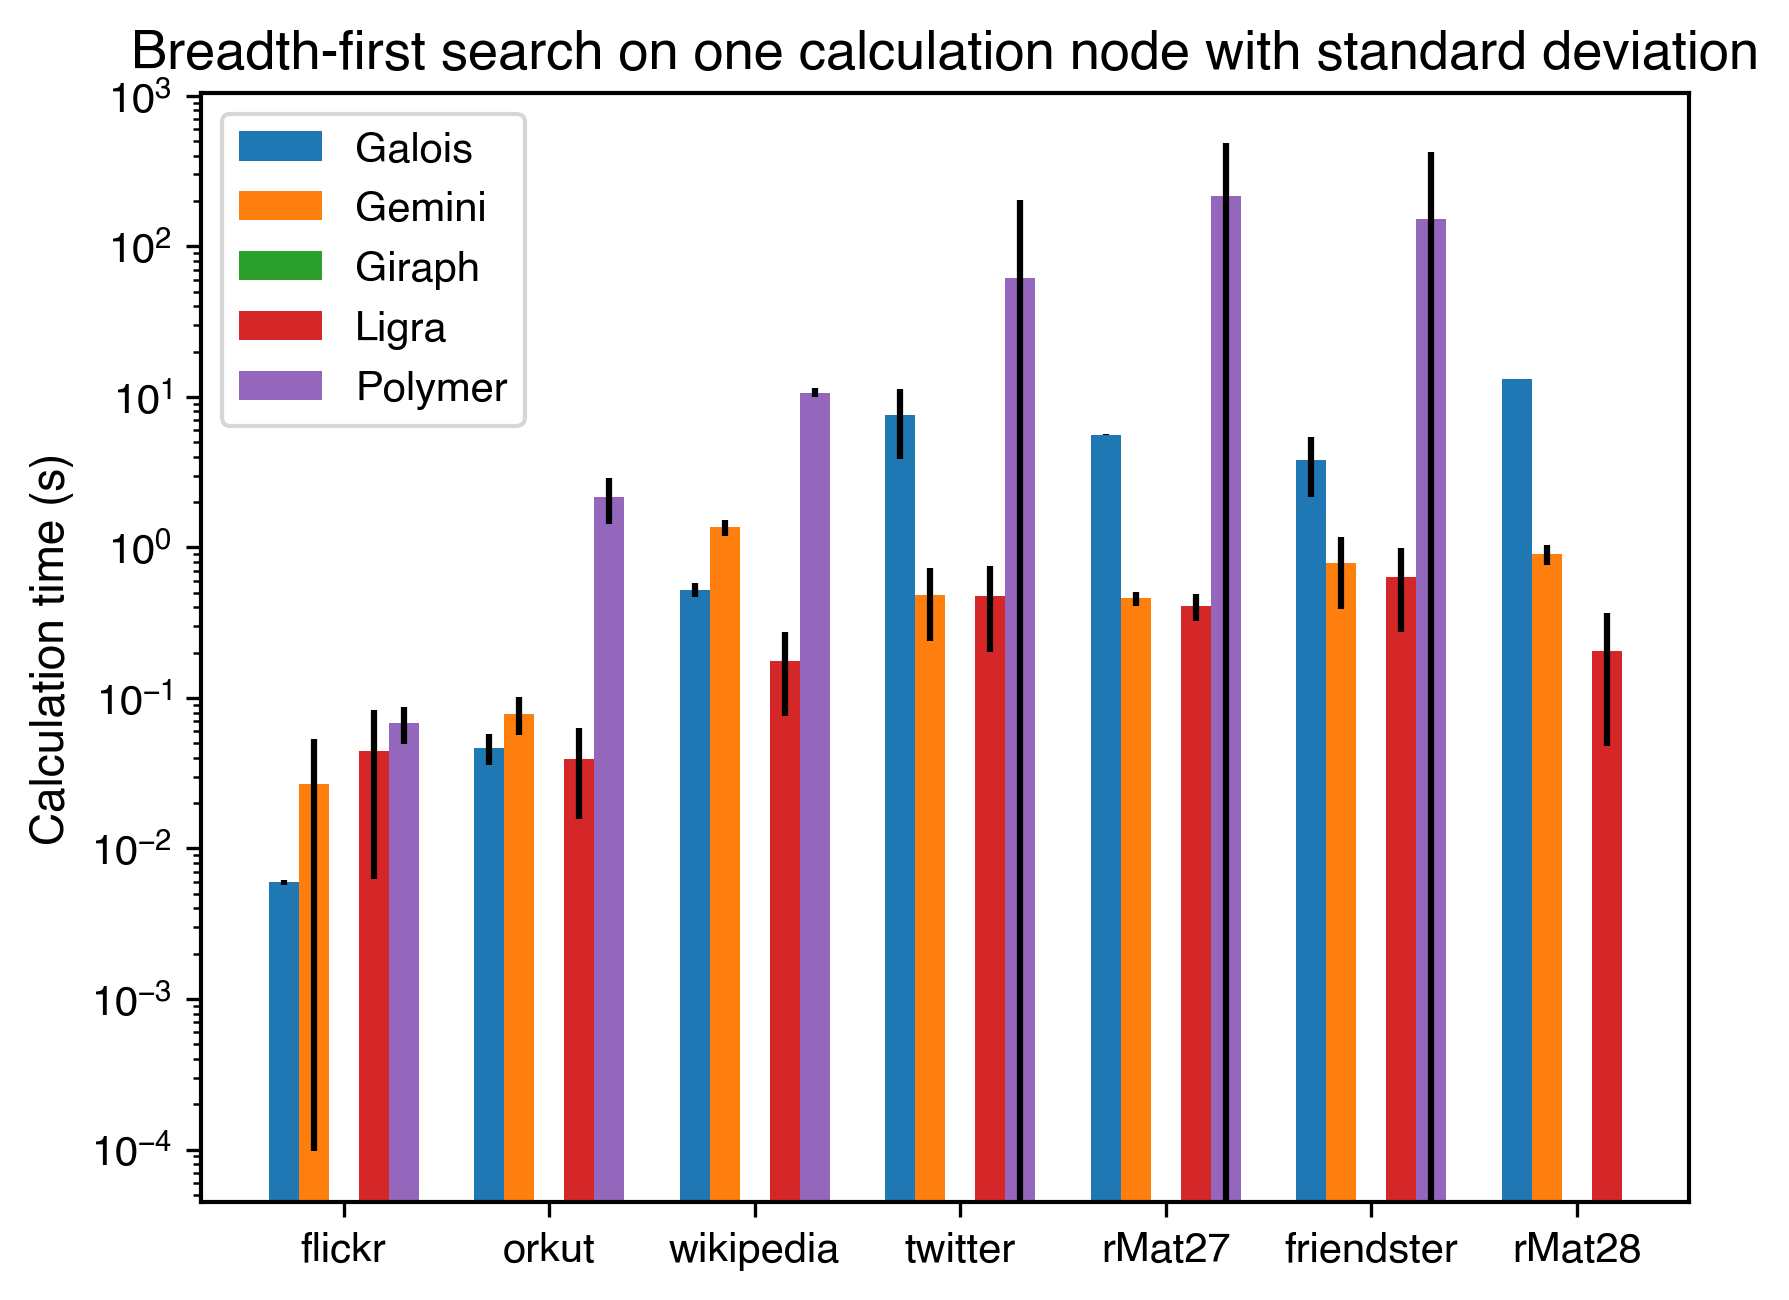
\includegraphics[width=\linewidth]{../../plots/singleNodeBFS_calcTime.png}
		\caption{Calculation time}
		\label{fig:singleNodeBFS_calc}
	\end{subfigure}
	\hfil
	\begin{subfigure}{0.32\textwidth}
		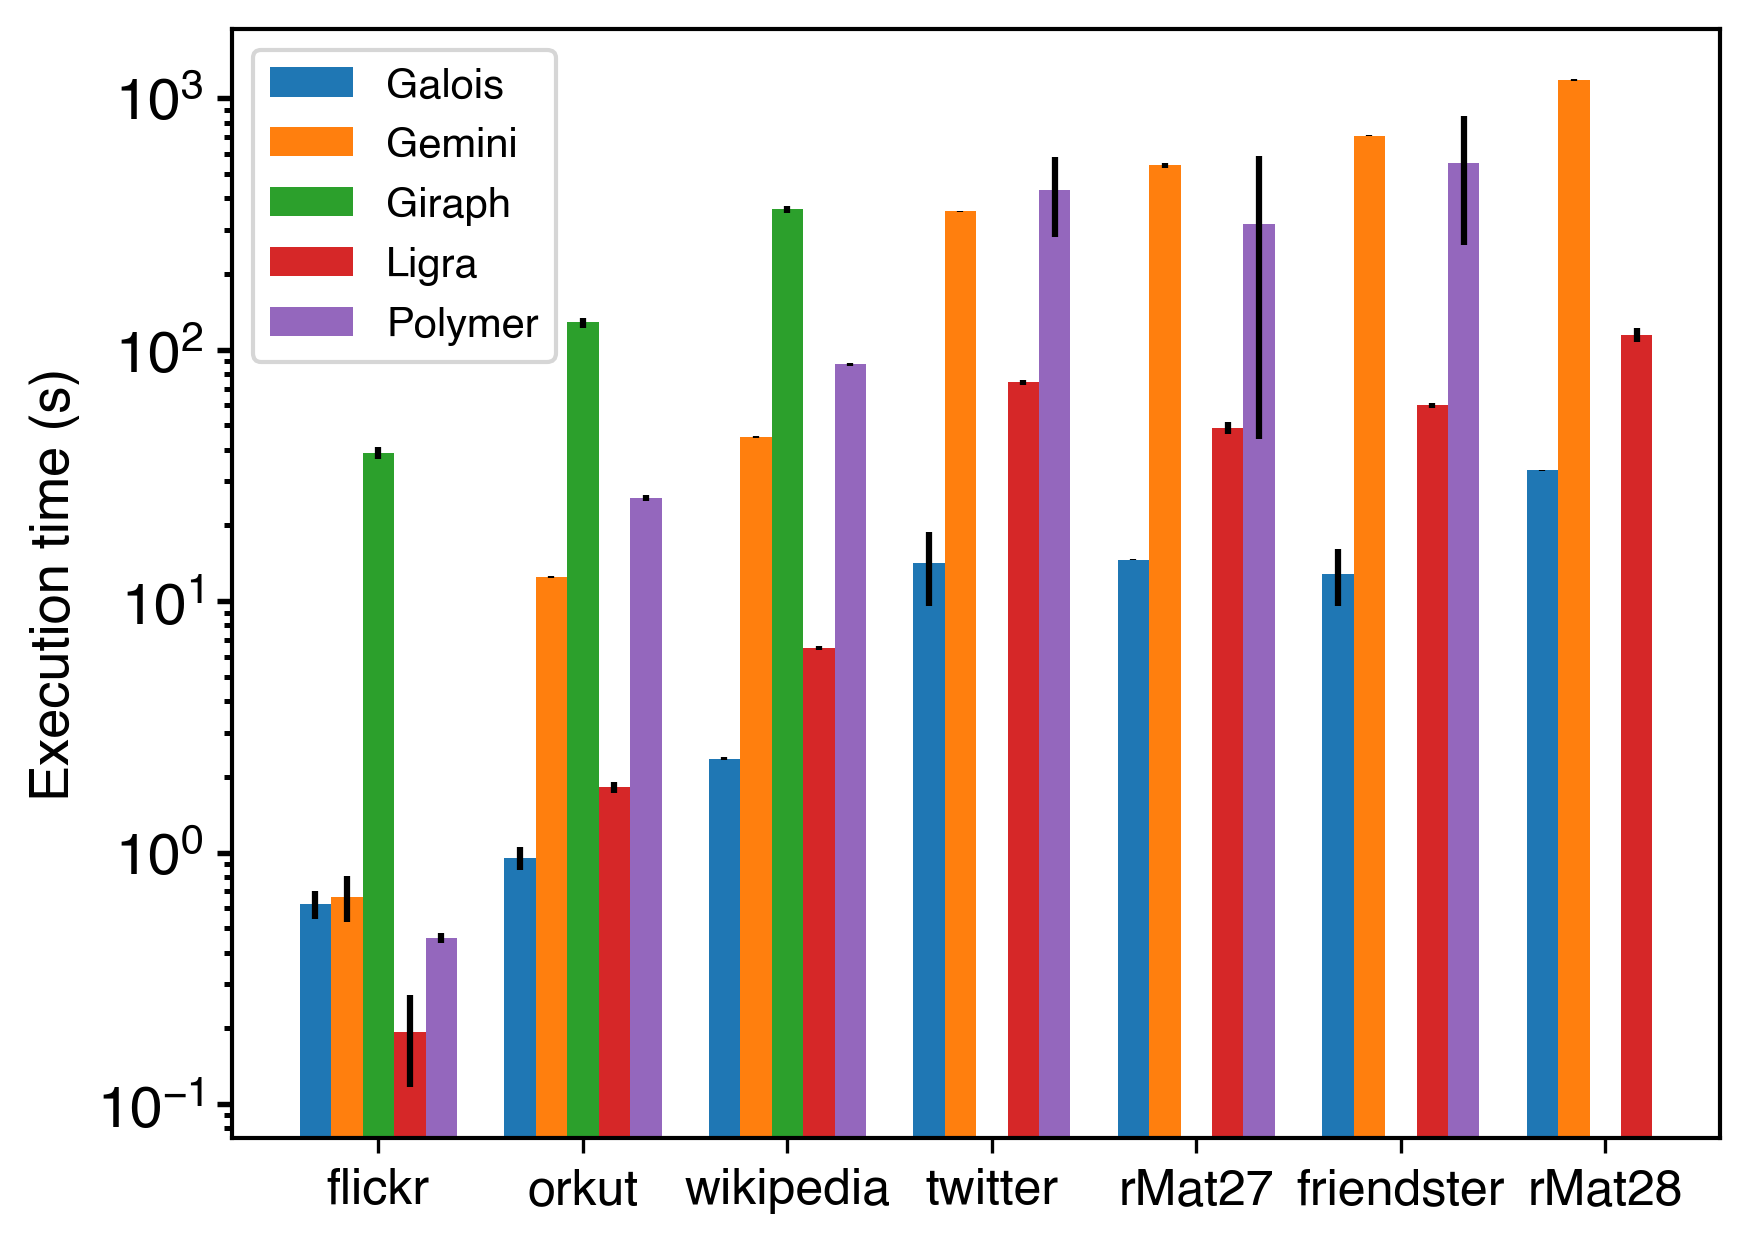
\includegraphics[width=\linewidth]{../../plots/singleNodeBFS_execTime.png}
		\caption{Execution time}
		\label{fig:singleNodeBFS_exec}
	\end{subfigure}
	\hfil
	\begin{subfigure}{0.32\textwidth}
		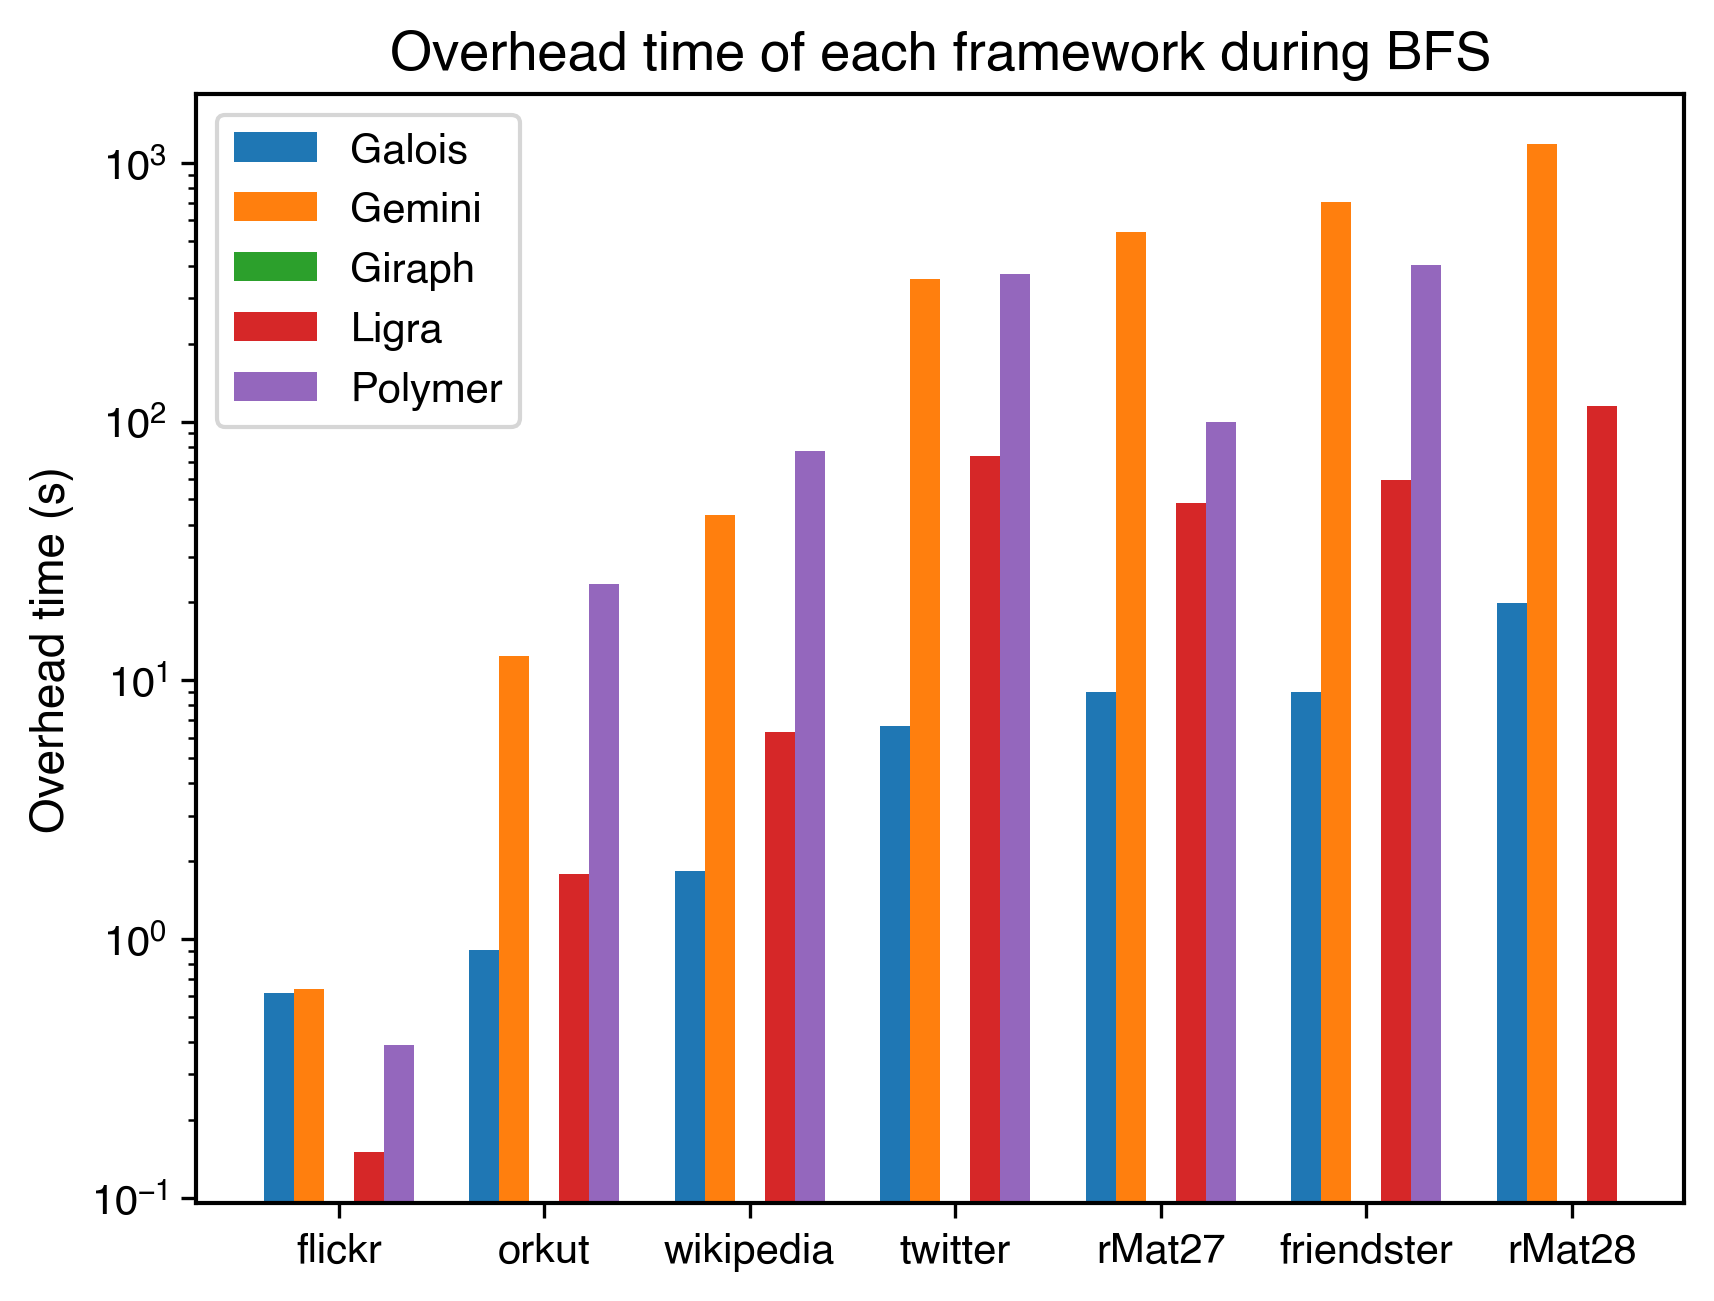
\includegraphics[width=\linewidth]{../../plots/singleNodeBFS_overheadTime.png}
		\caption{Overhead time}
		\label{fig:singleNodeBFS_overheadNormalized}
	\end{subfigure}
	\caption{Average times for BFS on a single computation node}
\end{figure*}
Giraph ran out of memory ($>$250 GB) on any graph larger than wikipedia. Also, Polymer failed to complete on rMat28. Ligra, that failed during SSSP however completed our benchmark for BFS.

The calculation times provided in \autoref{fig:singleNodeBFS_calc} show Gemini and Ligra to be comparable in their performance. 
Their computation times deviate less than 151ms on all graphs except wikipedia and rMat28, with Ligra being the faster framework on most graphs.
Ligra is between 2ms (twitter) and 151ms (friendster) faster than Gemini.
In turn, Gemini is 17ms faster than Ligra on flickr.
Only on wikipedia and rMat28, there is a noticeable difference between the two frameworks. Ligra is 1.2s (7.8$\times$) faster than Gemini on wikipedia and 696ms (4.4$\times$) faster on rMat28.

We compare the remaining frameworks to Ligra because it is generally slightly faster than Gemini.
Giraph and Polymer are one to two orders of magnitude slower. The only exception to this is Polymer on flickr, here Polymer is just 24ms (35\%) slower than Ligra.
Giraph takes between 13$\times$ and 32$\times$ longer than Ligra on flickr, orkut or wikipedia.
As already stated, Polymer is comparable to Ligra on flickr, but for the other graphs, its calculation times are even longer than those of Giraph. However, Polymer managed -- contrary to Giraph -- to finish computation on some larger graphs.
Polymer takes between 55$\times$ and 530$\times$ longer than Ligra on the graphs larger than flickr.
Here, the difference between the times of rMat27 and friendster are especially interesting. There are 20\% (439M) more edges in friendster, yet the computation for the synthetic rMat27 takes 42\% longer.
Galois calculation performance is comparable to Gemini or Ligra on the smaller three graphs (flickr, orkut and wikipedia).
Only on the larger graphs is Galois slower than Gemini or Ligra, meanwhile Galois is always faster than Polymer by one order of magnitude.

The execution time results are very similiar to our findings of SSSP (cf. \autoref{fig:singleNodeSSSP_exec}). Just like on SSSP, Galois is the fastest framework and Ligra is second fastest on all graphs except flickr.
Again, Gemini and Polymer are comparable in their performance and at the same time the slowest frameworks on all graphs except flickr, orkut and wikipedia.
On those three graphs, Giraph is the slowest, by a difference of one to two orders of magnitude compared to Galois.
On the other graphs, Polymer and Gemini are one order of magnitude slower than Galois.

\paragraph{Distributed}
\begin{figure*}
	\hfil
	\begin{subfigure}{0.32\textwidth}
		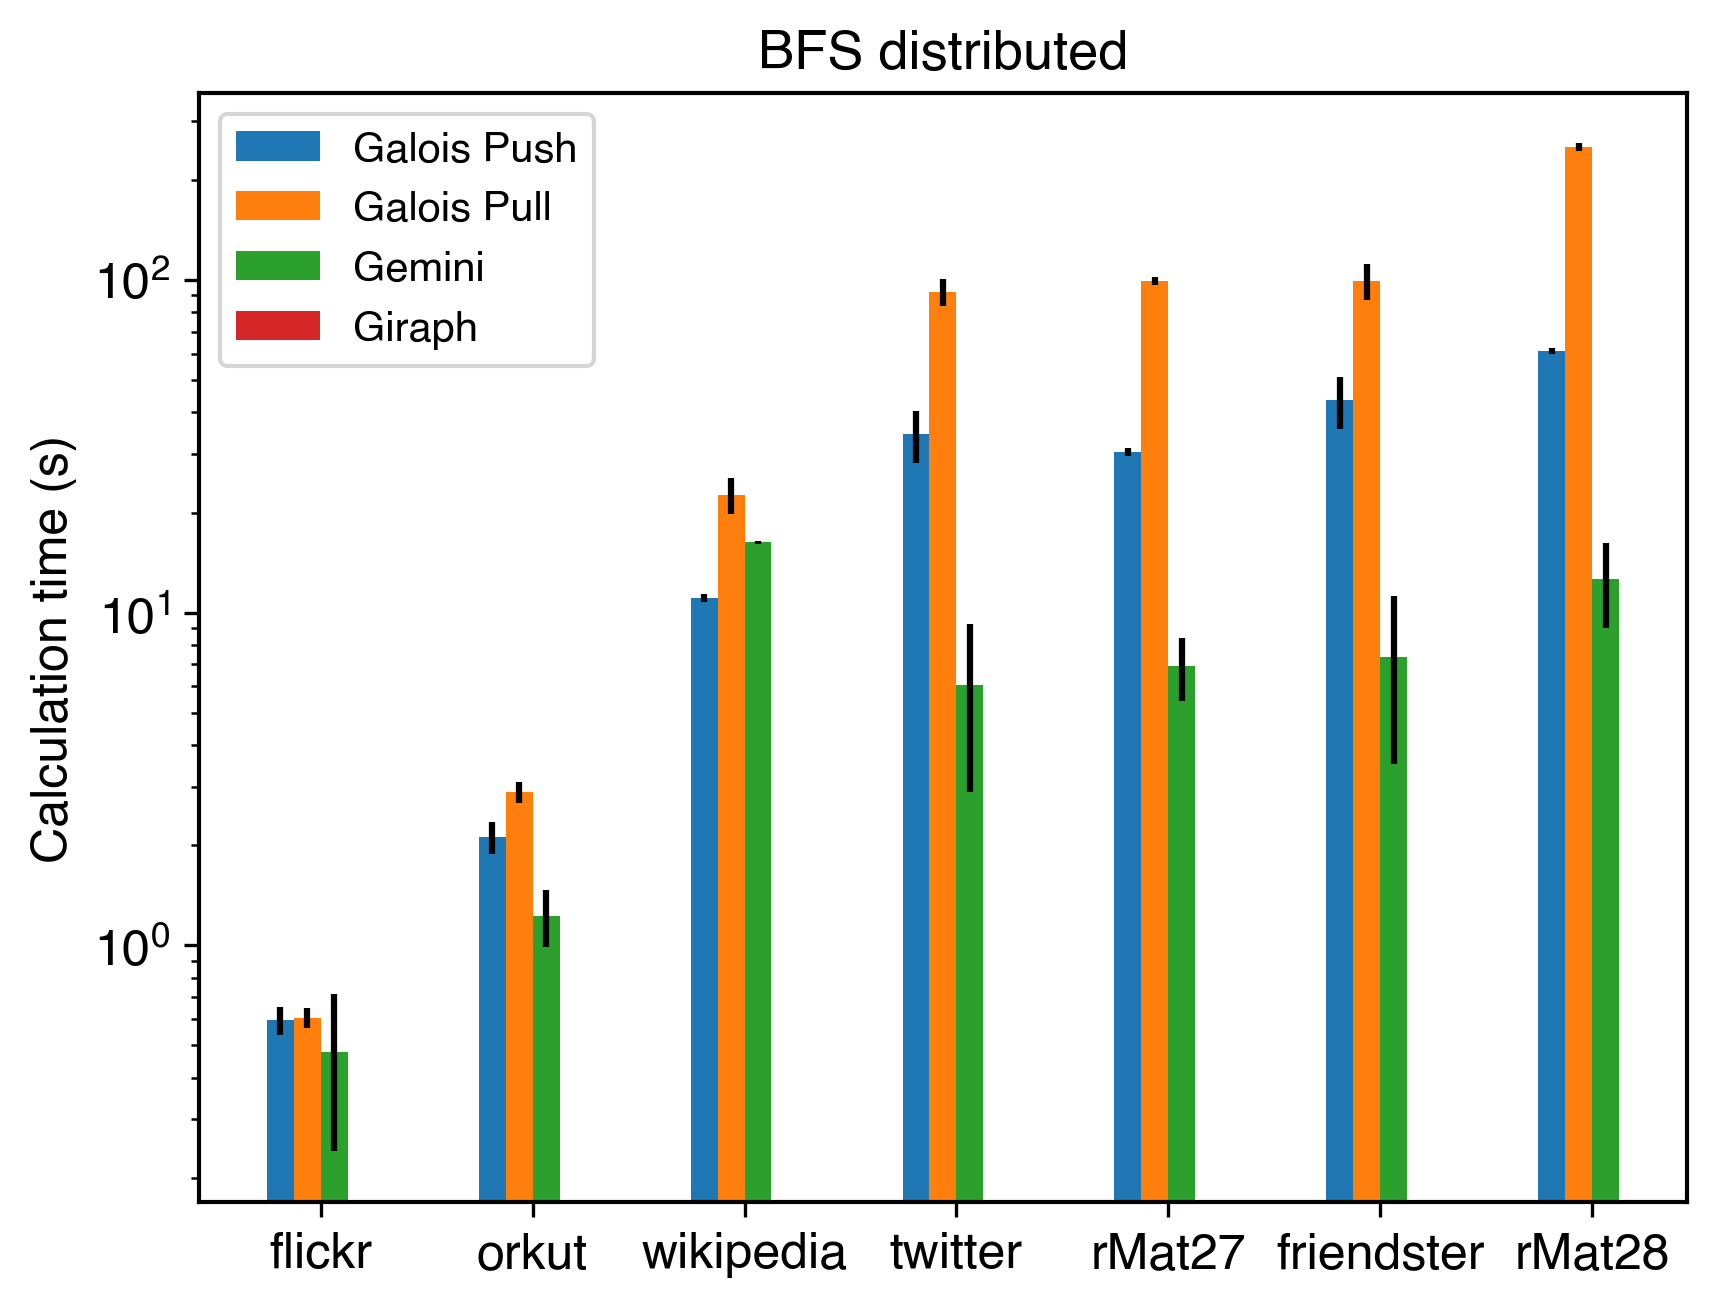
\includegraphics[width=\linewidth]{../../plots/distributedBFS_calcTime.png}
		\caption{Calculation time}
		\label{fig:distributedBFS_calc}
	\end{subfigure}
	\hfil
	\begin{subfigure}{0.32\textwidth}
		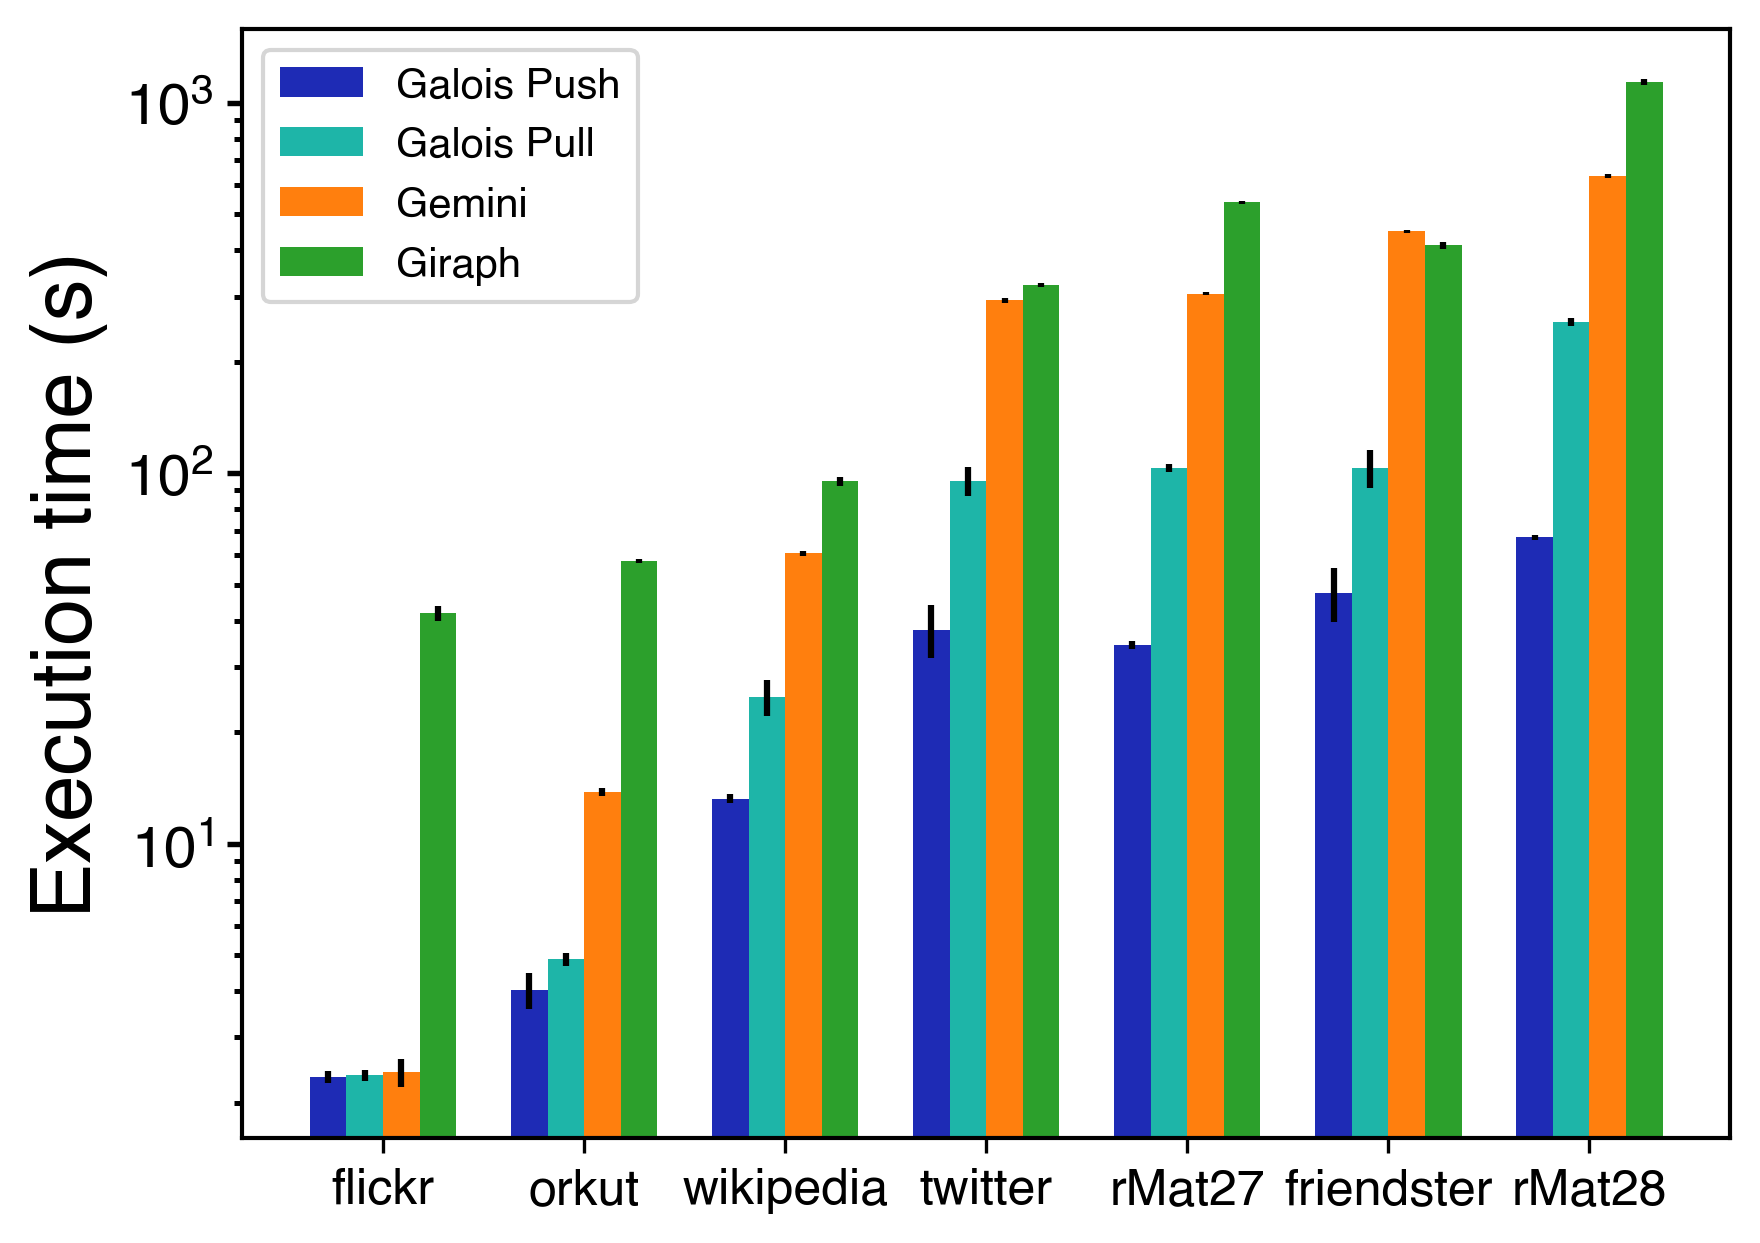
\includegraphics[width=\linewidth]{../../plots/distributedBFS_execTime.png}
		\caption{Execution time}
		\label{fig:distributedBFS_exec}
	\end{subfigure}
	\hfil
	\begin{subfigure}{0.32\textwidth}
		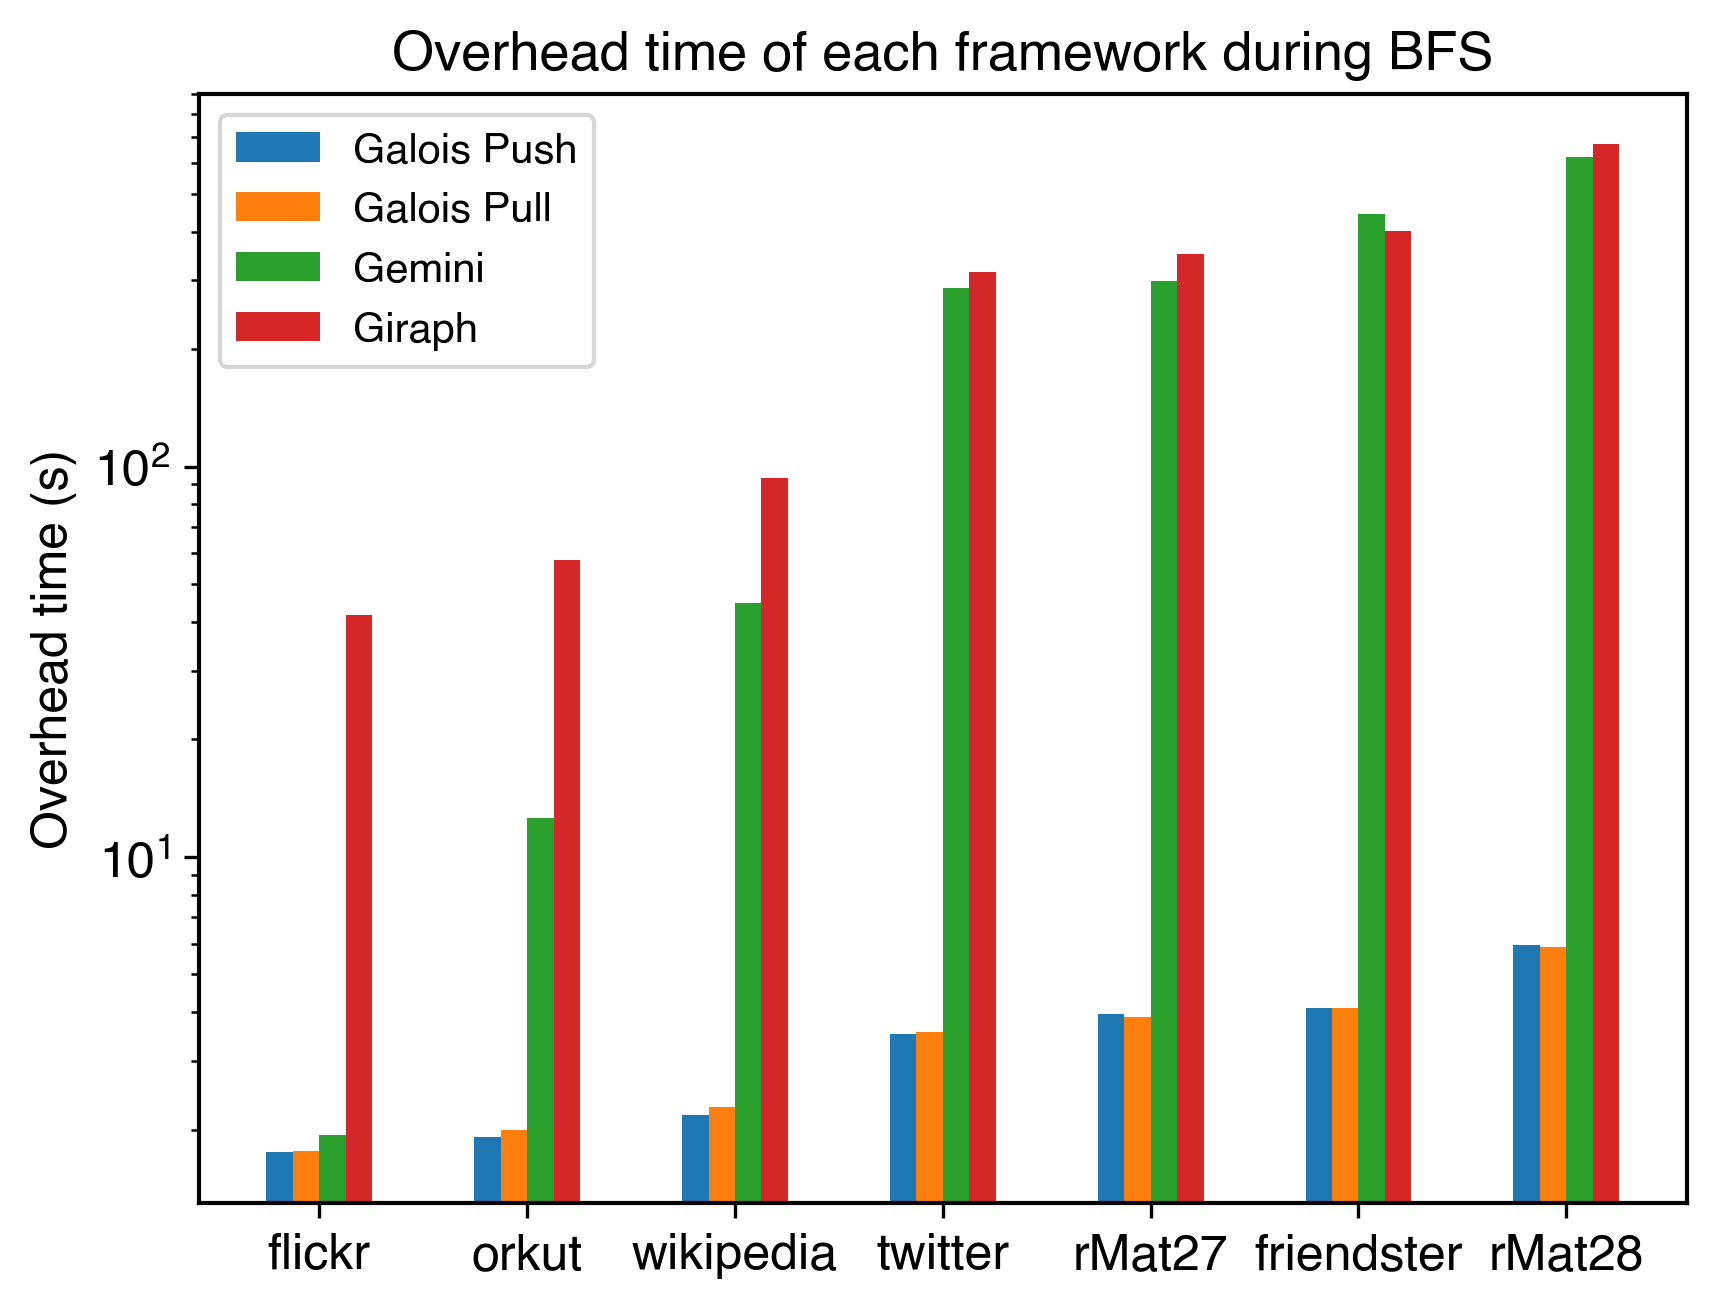
\includegraphics[width=\linewidth]{../../plots/distributedBFS_overheadTime.png}
		\caption{Overhead}
		\label{fig:distributedBFS_overhead}
	\end{subfigure}
	\hfil
	\caption{Average times for BFS on the distributed cluster}
	\label{fig:distributedBFS}
\end{figure*}
For both the calculation and the execution times, Breadth-First Search shows similar behaviour as the distributed SSSP test case. This is expected since both are graph traversal algorithms starting in one source vertex.
Hence, calculation complexity for each vertex and communication overhead is comparable. All measurements can be seen in \autoref{fig:distributedBFS}.

The results for calculation time (cf. \autoref{fig:distributedBFS_calc}) show Giraph to have very short calculation times on the real-world graphs, while Giraph's calculation times on both rMat27 and rMat28 are the worst of all frameworks. Thus, Giraph is fastest on the three smallest graphs and second fastest on twitter and friendster. On those two graphs, Gemini is fastest with only a small margin between the two frameworks.
Just like with SSSP, the Galois implementations have the longest calculation time on the real-world graphs. And Galois is second slowest, on the synthetic graphs.

Comparing the execution times in \autoref{fig:distributedBFS_exec} results again in similar findings to SSSP.
While Gemini can compete with Galois on the small flickr graph, moving to larger data sets shows the worse performance of Gemini compared to Galois.
Similar to SSSP, Giraph is slowest on all but one graph. Only on friendster is Gemini marginally slower, this was also the case for SSSP.
Galois Push is generally faster than the Pull alternative while both Push and Pull versions are faster than Gemini and Giraph across all graphs.
This makes Galois Push the clear winner for distributed BFS.

